

%----------------------------------------------------------------------------------------
%	PACKAGES AND OTHER DOCUMENT CONFIGURATIONS
%----------------------------------------------------------------------------------------

\documentclass[12pt]{article} 
 
\usepackage{polski}
\usepackage[polish]{babel}
\usepackage[utf8]{inputenc}
\usepackage{datetime}
\usepackage{graphicx}
\usepackage{tikz} 
\usepackage{amsmath}
\usepackage{epstopdf}
\usepackage{array,booktabs} 
\usepackage{float}
%\usepackage[colorlinks=true]{hyperref}
%\usepackage[all]{hypcap}
%\usepackage{showframe}
\usepackage{geometry}
 \geometry{
 a4paper, 
 left=30mm,
 right=30mm,
 top=30mm,
 bottom=30mm,
 }
 
\newdate{create_date}{02}{06}{2014}

%----------------------------------------------------------------------------------------

%----------------------------------------------------------------------------------------
% TIKZ PACKAGES
%----------------------------------------------------------------------------------------

\usetikzlibrary{arrows, calc}

%----------------------------------------------------------------------------------------

\begin{document}

\begin{titlepage}

\newcommand{\HRule}{\rule{\linewidth}{0.5mm}}
% Defines a new command for the horizontal lines, change thickness here

\center
% Center everything on the page
 
%----------------------------------------------------------------------------------------
%	LOGO SECTION
%----------------------------------------------------------------------------------------


\includegraphics[width=6cm]{../res/img/logo.png}\\[1cm]
% Include a department/university logo - this will require the graphicx package
 
%----------------------------------------------------------------------------------------
 
%----------------------------------------------------------------------------------------
%	HEADING SECTIONS
%----------------------------------------------------------------------------------------

\textsc{\LARGE Akademia Górniczo-Hutnicza \\[0.2cm]
im. Stanisława Staszica w Krakowie}\\[1.5cm]
% Name of your university/college

\textsc{\Large Podstawy Automatyki}\\[0.5cm]
% Major heading such as course name

%----------------------------------------------------------------------------------------
%	TITLE SECTION
%----------------------------------------------------------------------------------------

\HRule \\[0.5cm]
{ \huge \bfseries Dyskretne układy regulacji \\[0.3cm] oraz \\[0.5cm] Analiza
serwomechanizmu \\[0.2cm] przekaźnikowego z wykorzystaniem płaszczyzny
fazowej}\\[0.3cm]
% Title of your document
\HRule \\[1.5cm]
 
%----------------------------------------------------------------------------------------
%	AUTHOR SECTION
%----------------------------------------------------------------------------------------

% \begin{minipage}{0.4\textwidth}
% \begin{flushleft} \large
% \emph{Author:}\\
% Konrad \textsc{Adasiewcz} % Your name
% \end{flushleft}
% \end{minipage}
% ~
% \begin{minipage}{0.4\textwidth}
% \begin{flushright} \large
% \emph{Supervisor:} \\
% dr inż. Paweł \textsc{Rotter} % Supervisor's Name
% \end{flushright}
% \end{minipage}\\[4cm]

% If you don't want a supervisor, uncomment the two lines below and remove the section above
\flushright
\Large \emph{Autorzy:}\\
Konrad \textsc{Adasiewcz}\\[0.1cm] % Your name
Michał \textsc{Maciejewski}\\[3cm] % Your name

%----------------------------------------------------------------------------------------
%	DATE SECTION
%----------------------------------------------------------------------------------------
Data wykonania ćwiczenia: \\
{\large \displaydate{exercise_date}}\\[1cm]


\vfill % Fill the rest of the page with whitespace

\end{titlepage}

\section{Wstęp}

Obiekty rzeczywiste są z reguły obiektami wysokiego rzędu, w związku z tym
trudne jest odnalezienie ich dokładnego modelu matematycznego. Dlatego
obiekty wysokich rzędów z reguły aproksymujemy obiektami niskich rzędów z
opóźnieniem. Jednak ponieważ model czystego opóźnienia transportowego w
dziedzinie transmitancji operatorowej, nie jest wyrażony skończonym ułamkiem
wymiernym jest to model wysoce niewygodny do analizy np. stabilnościowej. W celu
umożliwienia przeprowadzenia takiej analizy przy pomocy narzędzi klasycznej
teorii sterowania, wykonuje się aproksymację członu opóźniającego. Jednym z
takich przybliżeń jest aproksymacja Pade.

\subsection{Aproksymacja Pade'go}

Aproksymacja Pade'go polega na przybliżeniu dowolnej funkcji różniczkowalnej
$n=m+k$ krotnie przy pomocy ułamka wymiernego postaci:

\begin{equation*}
	F(x) = \frac{a_0+a_1x+\ldots +a_kx^k}{b_0+b_1x+\ldots +b_mx^m}
\end{equation*}

Funkcja $F$ jest aproksymacją Pade'go funkcji $f$ jeśli spełnia warunki:

\begin{equation*}
	\begin{cases}
		F(x_0) & = f(x_0) \\[0cm]
		F^{(i)}(x_0) & =
		f^{(i)}(x_0) \hspace{0.5cm} i=1,\ldots n
	\end{cases}
\end{equation*}

Bez utraty ogólności można założyć iż $x_0=0$, oraz iż $b_0=1$ lub $a_0=1$.

\section{Aproksymacja członu opóźniającego}

Nazwijmy aproksymację Pade'go funkcji $f(s)=e^{-s\tau}$ rzędu $2n$ o
jednakowych rzędach licznika i mianownika aproksymacją członu opóźniającego
rzędu $n$. Wtedy aproksymacje członu opóźniającego rzędów 1 oraz 2 mają postać
jak niżej:

\begin{equation*}
	\begin{cases}
		F_1(s) & = \dfrac{1-\frac{\tau}{2}s}{1+\frac{\tau}{2}s} \\[0.5cm]
		F_2(s) & = \dfrac	{1-\frac{\tau}{2}s+\frac{\tau^2}{12}s^2}
							{1+\frac{\tau}{2}s+\frac{\tau^2}{12}s^2}
		\\[0cm]
	\end{cases}
\end{equation*}

\newpage

\begin{figure}[!htb]
	\begin{center}
		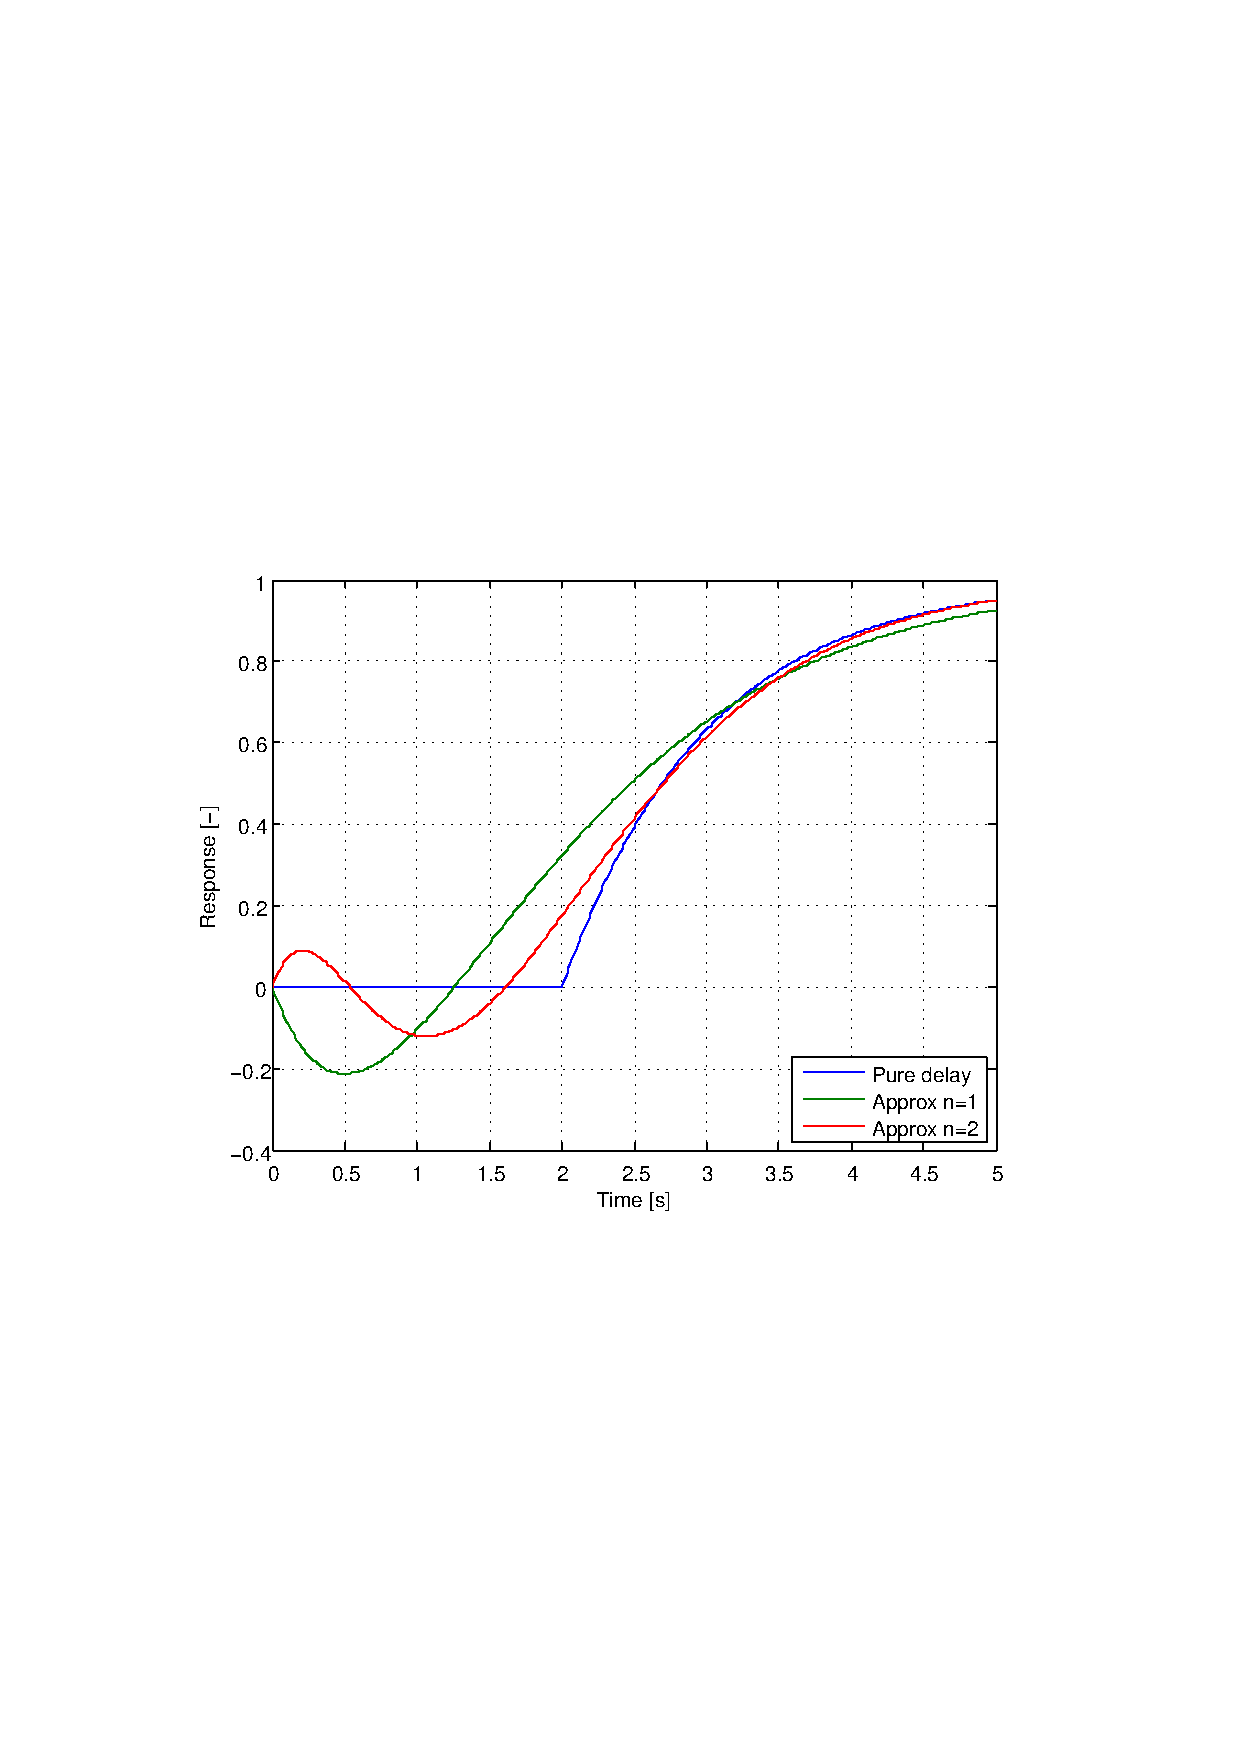
\includegraphics[width=14cm,trim=3cm 9cm 3cm 9cm,clip]
		{../res/img/pade1_2.pdf}
	\end{center}
	\caption{Odpowiedzi skokowe obiektu inercyjnego pierwszego rzędu z czystym
	opóźnieniem, oraz jego aproksymacjami}
\end{figure}

Jak widać, aproksymata opóźnienia powoduje oscylacje o niewielkiej amplitudzie,
których liczba rośnie a amplituda maleje wraz ze wzrostem rzędu aproksymacji.

\newpage

\section{Aproksymacja układu wysokiego rzędu przez układ niskiego rzędu z
opóźnieniem}

W celu dopasowania do próby, modelu niskiego rzędu z opóźnieniem, parametry
transmitancji dopiera się najpierw empirycznie. Aproksymujemy obiekt inercyjny
10 rzędu o transmitancji:

\begin{equation*}
	G(s)=\frac{1}{(0.2s+1)^{10}}
\end{equation*}

Przyjęty model jest modelem drugiego rzędu z opóźnieniem o transmitancji:

\begin{equation*}
	G(s)=D_k(s)\frac{1}{as^2+bs+1}
\end{equation*}

gdzie $D_k(s)$ jest transmitancją aproksymacji członu opóźniającego
rzędu $k$-tego.

Odpowiedź skokowa modelu przy ręcznie dobranych parametrach na tle odpowiedzi
modelowanego obiektu prezentują się następująco:

\begin{figure}[!htb]
	\begin{center}
		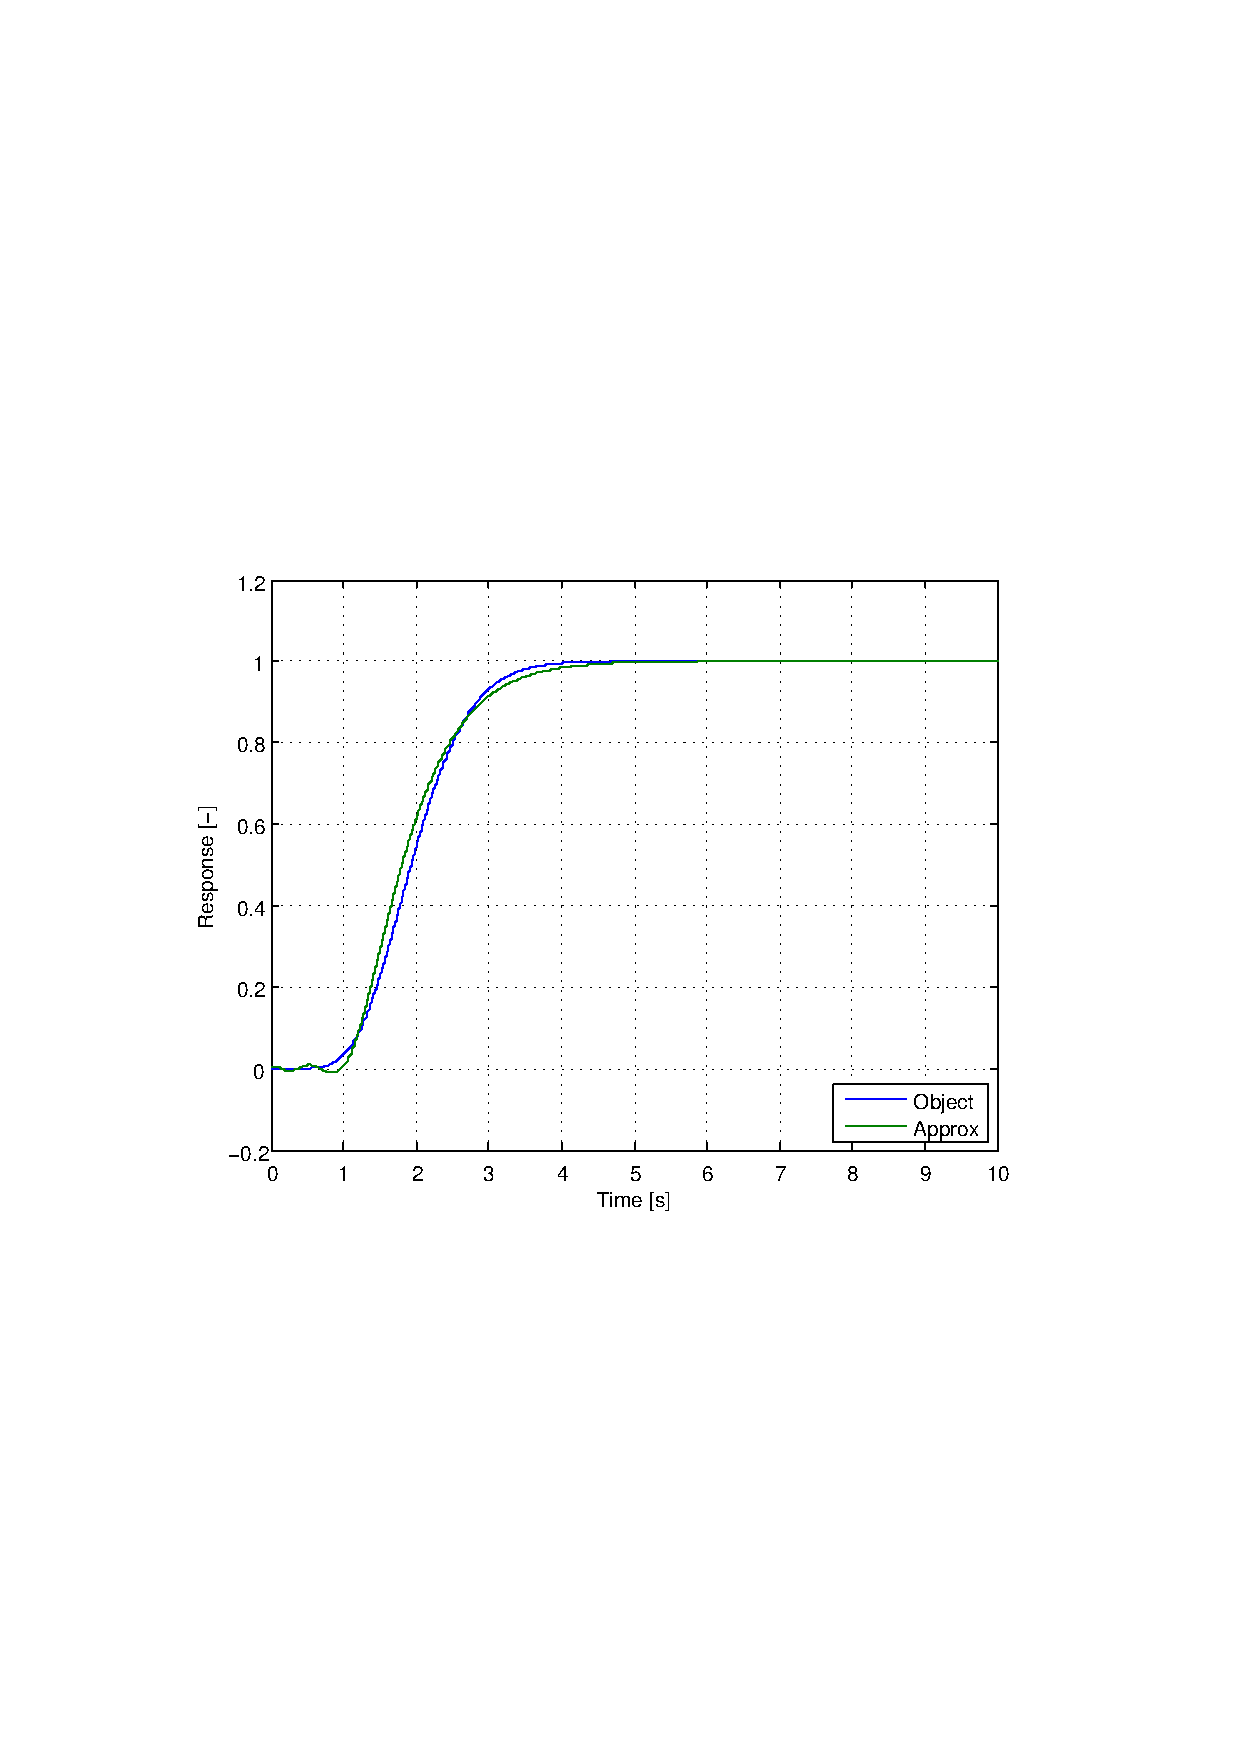
\includegraphics[width=14cm,trim=3cm 9cm 3cm 9cm,clip]
		{../res/img/modelfit_h.pdf} 
	\end{center}
	\caption{Odpowiedzi skokowe obiektu badanego, oraz jego aproksymacji dla
	parametrów $a=0.25$, $b=1$, $\tau=1$, $n=4$}
\end{figure}

Całka z kwadratu błędu za okres pomiaru ma wartość dla tak dobranych parametrów
$\varepsilon=0.00509$.

\newpage

Wykorzystując funkcję \textsc{Matlab}-a \textit{fminsearch} można w prosty
sposób uzyskać wartości parametrów $a$, $b$, $\tau$ minimalizujące dowolną
funkcję z nimi związaną. My minimalizujemy całkę z kwadratu błędu. Wyszukane w
ten sposób parametry dają wartość błędu aproksymacji za okres pomiaru równy
$\varepsilon=0.00066$. Poniżej odpowiedź skokowa obiektu i dopasowanego modelu.

\begin{figure}[!htb]
	\begin{center}
		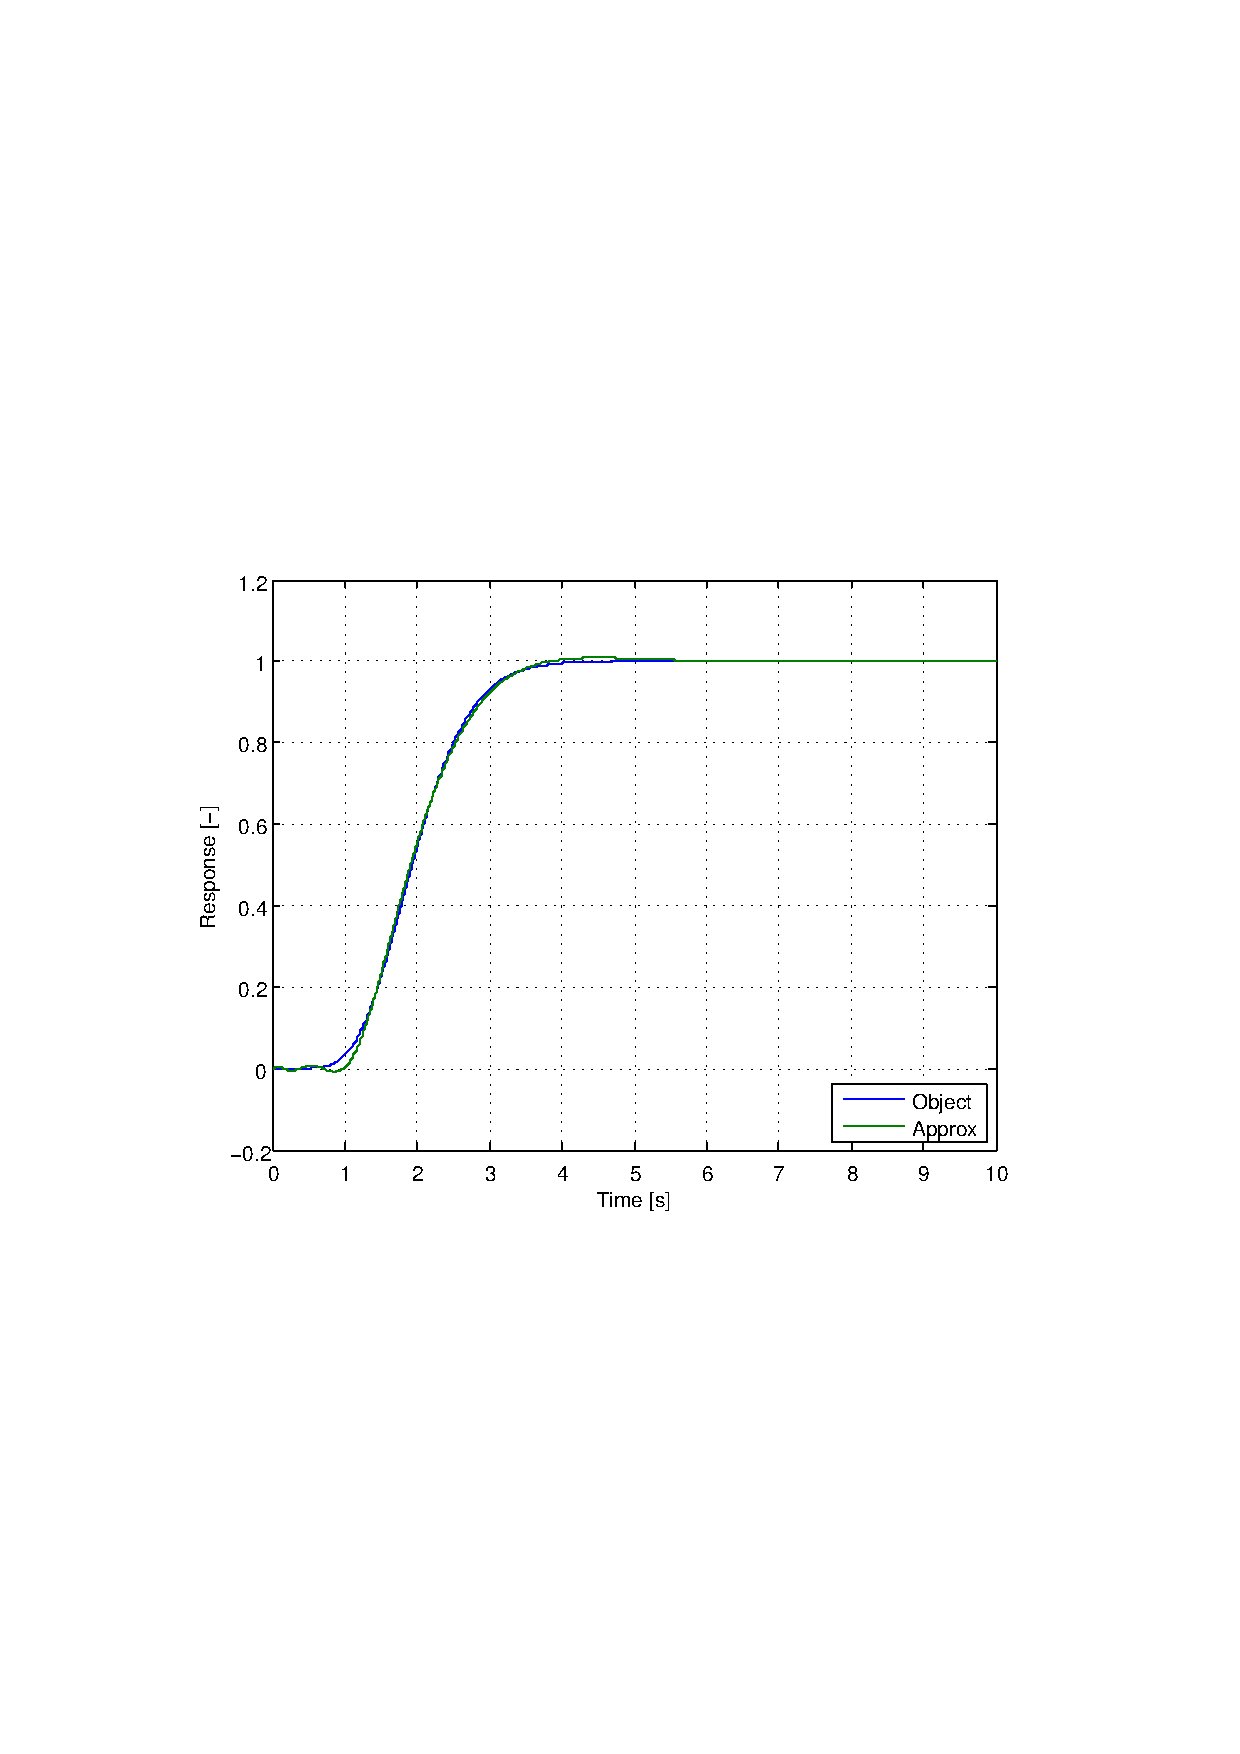
\includegraphics[width=14cm,trim=3cm 9cm 3cm 9cm,clip]
		{../res/img/modelfit_a.pdf} 
	\end{center}
	\caption{Odpowiedzi skokowe obiektu badanego, oraz jego aproksymacji dla
	parametrów $a=0.38$, $b=1.03$, $\tau=0.97$, $n=4$}
\end{figure}

\section{Wnioski i spostrzeżenia}

Rzeczywiste obiekty dynamiczne są obiektami wysokich rzędów, można jednak
przybliżać je modelami niższych rzędów sprowadzając różnicę odpowiedzi skokowych
do minimum. Jednak większość obiektów rzeczywistych to obiekty zachowujące się
jak obiekty z opóźnieniem, co stanowi pewną trudność w kwestii analizy
matematycznej takich modeli, ponieważ człon idealny człon opóźniający nie jest
opisany transmitancją w postaci ułamka wymiernego. W tym celu stosuje się
aproksymację Pade'go, dzięki której analizę transmitancji można przeprowadzić
stosując metody klasycznej teorii sterowania.

\end{document}